\subsection{K562 cell line} \label{meth-encode-k562-subsect}
After data pre-processing, we applied EM algorithm for clustering DNA methylation profiles for the K562 cell line. As promoter regions were considered $500bp$ upstream and $500bp$ downstream of the TSS, resulting in $1,000bp$ in total. This resulted in $5,270$ promoter regions for testing. The total number of clusters K was set to 5, and the methylation profiles were modelled using $5^{th}$ degree polynomials. 

\emph{Fig. \ref{methk562:first}} depicts the five latent functions $\mathbf{f}$ (\ie clusters) that were fitted to the K562 data after running EM algorithm. The \emph{y-axis} denotes the methylation level, and the \emph{x-axis} denotes the CpG locations in the promoter region scaled to the $[-1, 1]$ interval. We observe that each cluster has captured a different methylation pattern. Unsurprisingly, about 65\% of the promoter regions were assigned to cluster $k=4$ (\emph{red curve}), which denotes unmethylated promoter regions. The remaining four clusters had around the same percentage of assignments. From a biological viewpoint, this is expected since promoter regions of mammalian genomes are rich of CpG islands (CGIs) \citep{Illingworth2009}, which are mostly unmethylated. 

To investigate the association between methylation patterns at gene promoters and gene expression, we used the corresponding RNA-Seq data to observe the expression levels of the protein-coding genes assigned to each cluster $k$, which are shown as \emph{boxplots} in \emph{Fig. \ref{methk562:second}}. Each coloured boxplot represents the expression level (\emph{y-axis}) of genes assigned to each cluster $k$ (\emph{x-axis}). 

Comparing the two figures we observe some functional role of the methylation patterns, which are also confirmed by previous studies, such as \citet{Vanderkraats2013}. For example, hyper-methylation of promoter regions is a generally accepted mechanism for silencing gene expression. On the other hand, unmethylated promoter regions are associated with high transcription activity \citep{Deaton2011}. Finally, we observe that the U-shape of cluster $k=5$ (\emph{green curve}) around the TSS is also associated with higher transcriptional activity compared to all the other clusters, excluding cluster $k=4$ which contains the unmethylated CpGs.
\begin{figure}[ht!]
     \begin{center}
        \subfigure[]{
            \label{methk562:first}
            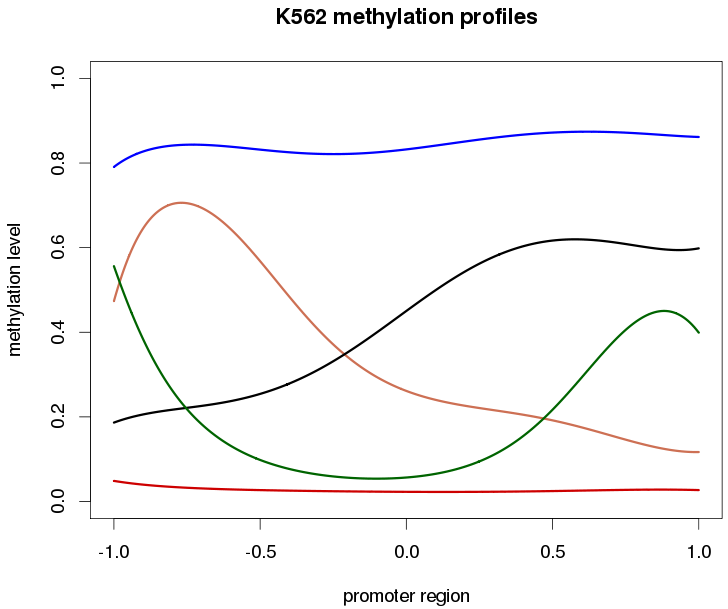
\includegraphics[width=0.45\textwidth]{images/k562MethProfClusters-2}
        }
        \subfigure[]{
           \label{methk562:second}
           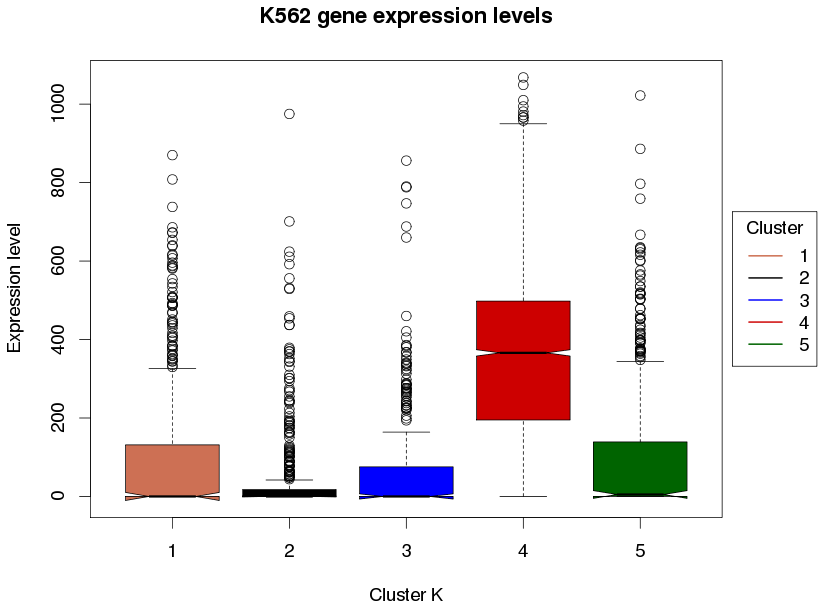
\includegraphics[width=0.51\textwidth]{images/k562MethProfBoxPlot-2}
        }
    \end{center}
    \caption{\emph{(a) Clustering DNA methylation profiles for the K562 cell line with $5^{th}$ degree polynomial. Each colour represents a different cluster. (b) Boxplot with the corresponding gene expression levels of the protein-coding genes assigned to each cluster K for the K562 cell line. See the text for details.}}
   \label{meth-k562-pic}
\end{figure}
